\chapter{Аналитический раздел}

Управление памятью вычислительной системы выполняется на трёх уровнях. 

\begin{enumerate}[label*=\arabic*.]
	\item Аппаратное обеспечение управления памятью (MMU, ОЗУ и т. д.).
	\item Управление памятью операционной системы (виртуальная память, защита).
	\item Управление памятью приложения (выделение и освобождение памяти, сборка мусора).
\end{enumerate}

Аппаратное обеспечение управления памятью состоит из электронных устройств и связанных с ними схем, которые хранят состояние вычислительной системы. К этим устройствам относятся регистры процессора, кэш, ОЗУ, MMU (Memory Management Unit, блок управления памятью) и вторичная (дисковая) память. Конструкция запоминающих устройств имеет решающее значение для производительности современных вычислительных систем. Фактически пропускная способность памяти является основным фактором, влияющим на производительность системы.~\cite{glossary}

Далее будет рассмотрено подробно управление памятью с точки зрения операционной системы и приложений.

\section{Управление памятью с точки зрения операционной системы}

\subsection{Иерархия памяти}

В процессе развития аппаратного обеспечения была разработана концепция \textbf{иерархии памяти}, согласно которой компьютеры обладают несколькими мегабайтами очень быстродействующей, дорогой и энергозависимой кэш-памяти, несколькими гигабайтами памяти, средней как по скорости, так и по цене, а также несколькими терабайтами памяти на довольно медленных, сравнительно дешевых дисковых накопителях, не говоря уже о сменных накопителях, таких как DVD и флеш-устройства USB. Превратить эту иерархию в абстракцию, то есть в модель, а затем управлять этой абстракцией --- и есть задача операционной системы. Та часть операционной системы, которая управляет иерархией памяти (или ее частью), называется \textbf{менеджером}, или \textbf{диспетчером}, \textbf{памяти}~\cite{tannenbaum}. Он должен следить за тем, какие части памяти используются, выделять память процессам, которые в ней нуждаются, и освобождать память, когда процессы завершат свою работу. Выбор, совершаемый менеджером памяти на этом этапе, может оказать существенное влияние на будущую эффективность программы, так как до 40\% (в среднем 17\%) времени её выполнения затрачивается на выделение и освобождение памяти.~\cite{cornell}

\subsection{Функции операционной системы по управлению памятью}

Помимо первоначального выделения памяти процессам при их создании операционная система должна также заниматься динамическим распределением памяти, то есть обслуживать запросы приложений на выделение им дополнительной памяти во время выполнения. После того, как приложение перестаёт нуждаться в дополнительной памяти, оно может вернуть её системе. Выделение случайного объёма памяти в случайные моменты времени из общего пула приводит к фрагментации памяти и, вследствие этого, к неэффективному её использованию. Дефрагментация памяти также является функцией операционной системы.

Таким образом, можно сформулировать следующие функции ОС по управлению памятью в мультипрограммных системах.

\begin{enumerate}[label*=\arabic*.]
	\item Отслеживание свободной и занятой памяти.
	\item Управление виртуальными адресными пространствами процессов, в том числе отображение виртуального адресного пространства процесса на физическую память.
	\item Динамическое распределение памяти. 
	\item Дефрагментация памяти. 
\end{enumerate}


\section{Управление памятью с точки зрения приложений}

\subsection{Среда выполнения языка программирования}

Менеджер памяти операционной системы с точки зрения выполняющихся на ней приложений обладает двумя серьёзными недостатками. Во-первых, он является недетерминированным: процессы не могут напрямую влиять на решения, принимаемые операционной системой по управлению их адресными пространствами. Во-вторых, менеджер памяти операционной системы не реализует те функции управления памятью, которые требуются конечному пользователю. Поэтому языки программирования реализуют собственную \textbf{среду выполнения} (language runtime), в которой реализуют необходимые пользователю функции для работы с памятью и создают собственные абстракции памяти.

Среда выполнения языка программирования может выполнять следующие функции:~\cite{dotnet_clr}

\begin{enumerate}[label*=\arabic*)]
	\item управление памятью;
	\item обработка исключений; 
	\item сборка мусора; 
	\item контроль типов;
	\item обеспечение безопасности; 
	\item управление потоками. 
\end{enumerate}

Управление потоками в среде выполнения языка подразумевает, что язык программирования организует многопоточное выполнение программы, используя возможности операционной системы, а также реализует некоторую \textbf{модель памяти}, которая для императивных языков программирования, поддерживающих многопоточное выполнение, определяет, какие записи в разделяемые переменные могут быть видны при чтениях, выполняемых другими потоками.~\cite{memory_model}

\subsection{Управление памятью}
\label{reference_locality}

Менеджер памяти приложения должен учитывать следующие ограничения.~\cite{mm_overview}

\begin{enumerate}[label*=\arabic*.]
	\item \textbf{Нагрузка на процессор} --- дополнительное время, затрачиваемое диспетчером памяти во время работы программы.
	\item \textbf{Блокировки} --- время, необходимое диспетчеру памяти для завершения операции и возврата управления программе. Это влияет на способность программы оперативно реагировать на интерактивные события, а также на любое асинхронное событие, например связанное с сетевым взаимодействием.
	\item \textbf{Накладные расходы памяти} --- дополнительный объём памяти, затрачиваемый на администрирование, а также накладные расходы, связанные с внутренней и внешней фрагментацией.
\end{enumerate}

Основная проблема управления памятью состоит в том, чтобы понять, когда следует сохранить содержащиеся в ней данные, а когда их следует уничтожить, чтобы память можно было использовать повторно. К сожалению, существует множество способов, которыми плохая практика управления памятью может повлиять на надежность и быстродействие программ, как при ручном, так и при автоматическом управлении памятью.

Ниже перечислены наиболее частые проблемы управления памятью.~\cite{mm_overview}

\begin{enumerate}[label*=\arabic*.]
	\item \textbf{Преждевременное освобождение памяти} (premature free). 
	Когда программы освобождают память, но позже пытаются получить к ней доступ, их поведение становится неопределённым. Сохранившаяся ссылка на освобождённую память называется \textbf{висячим указателем} (dangling pointer).
	\item \textbf{Утечки памяти} (memory leaks). Когда программы интенсивно выделяют память, не освобождая её, в конечном итоге память заканчивается.
	\item \textbf{Внешняя фрагментация} (external fragmentation). Работа аллокатора по выделению и освобождению памяти может привести к тому, что он больше не сможет выделять достаточно большие области памяти, несмотря на наличие достаточного общего количества свободной памяти. Это связано с тем, что свободная память может быть разделена на множество небольших областей, разделённых используемыми данными. Данная проблема особенно критична в серверных приложениях, работающих в течение длительного времени.
	\item \textbf{Неэффективное расположение ссылок} (poor locality of reference). Эта проблема связана с тем, как современные менеджеры памяти аппаратного обеспечения и операционной системы обращаются с памятью: последовательные обращения к памяти выполняются быстрее, если они производятся к соседним областям памяти. Если менеджер памяти разместит данные, которые программа будет использовать вместе, не в соседних областях памяти, то быстродействие программы уменьшится.
	\item \textbf{Негибкий дизайн} (inflexible design). Менеджеры памяти могут вызвать серьезные проблемы с производительностью, если они были разработаны с одной целью, а используются для другой. Эти проблемы вызваны тем, что любое решение по управлению памятью опирается на предположения о том, как программа будет использовать выделенную память. Например, на стандартные размеры областей памяти, шаблоны ссылок или время жизни объектов. Если эти предположения неверны, то диспетчер памяти может работать с памятью менее эффективно.
	\item \textbf{Межмодульное взаимодействие} (interface complexity). Если объекты передаются между модулями программы, то при проектировании интерфейсов модулей необходимо учитывать управление их памятью.
\end{enumerate}

Управление памятью приложения объединяет две взаимосвязанные задачи: выделение памяти (allocation) и её переиспользование (recycling), когда она больше не требуется. За выделение памяти отвечает \textbf{аллокатор}~\cite{allocator}. Его необходимость обусловлена тем, что процессы, как правило, не могут заранее предсказать, сколько памяти им потребуется, поэтому они нуждаются в реализации дополнительной логики обслуживания изменяющихся запросов к памяти. Решение об освобождении и переиспользовании выделенной аллокатором памяти, которая больше не используется приложением, может быть принято либо программистом, либо средой выполнения языка. Соответственно, в зависимости от этого управление памятью в языке программирования может считаться либо ручным, либо автоматическим.

\subsubsection{Ручное управление памятью}

При ручном управлении памятью программист имеет прямой контроль над временем жизни объектов программы. Как правило, он осуществляется либо явными вызовами функций управления кучей (например, malloc и free в C), либо языковыми конструкциями, влияющими на стек управления (например, объявлениями локальных переменных). Ключевой особенностью ручного менеджера памяти является то, что он даёт возможность явно указать, что заданная область памяти может быть освобождена и переиспользована.~\cite{mm_overview}

Преимущества ручного управления памятью: 

\begin{itemize}[label*=---]
	\item явное выделение и освобождение памяти делает программы более прозрачными для разработчика;
	\item ручные менеджеры памяти, как правило, используют память более экономно, так как программист может минимизировать время между моментом, когда выделенная память перестаёт использоваться, и её фактическим освобождением.
\end{itemize}

Недостатки ручного управления памятью: 

\begin{itemize}[label*=---]
	\item увеличение исходного кода программ за счёт того, что управление памятью, как правило, составляет значительную часть интерфейса любого модуля;
	\item повышение дублирования кода за счёт использования однотипных инструкций управления памятью;
	\item увеличение числа ошибок управления памятью из-за человеческого фактора.
\end{itemize}

К языкам с ручным управлением памятью относятся C, C++, Zig и другие. На таких языках программисты могут писать код, дублирующий поведение менеджера памяти либо путем выделения больших областей и их разделения для использования, либо путем внутреннего переиспользования этих блоков. Такой код называется \textbf{субаллокатором} (suballocator)~\cite{glossary}, так как он работает поверх другого аллокатора. Субаллокаторы могут использовать как преимущество специальные знания о поведении программы, но в целом они менее эффективны, чем использование базового аллокатора. Также стоит отметить, что субаллокаторы могут быть неэффективными или ненадежными, тем самым создавая новый источник ошибок.~\cite{allocator}

\subsubsection{Автоматическое управление памятью}

Автоматическое управление памятью, как правило, работает либо как часть среды выполнения языка, либо как расширение. Автоматические менеджеры памяти обычно перерабатывают области памяти, которые недоступны из переменных программы (то есть области, к которым невозможно получить доступ с помощью указателей). Задачи автоматического управления памятью:~\cite{mm_overview}

\begin{itemize}[label*=---]
	\item выделение памяти под новые объекты;
	\item идентификация используемых объектов;
	\item освобождение памяти, занятой неиспользуемыми объектами.
\end{itemize}

Преимущества автоматического управления памятью: 

\begin{itemize}[label*=---]
	\item освобождение разработчика от задачи управления памятью в своих программах;
	\item уменьшение объёма исходного программ за счёт отсутствия необходимости явно работать с памятью;
	\item уменьшение числа ошибок управления памятью;
	\item автоматическое управление памятью может быть более эффективным, чем ручное, за счёт применения соответствующих алгоритмов.
\end{itemize}

Недостатки автоматического управления памятью: 

\begin{itemize}[label*=---]
	\item время жизни объектов программы становится непрозрачным для разработчика, так как часть логики работы с памятью реализована на уровне языка;
	\item память, как правило, используется менее экономно, так как существует некоторая задержка между моментом, когда память перестаёт использоваться, и моментом её освобождения; такие задержки определяются алгоритмами автоматической переработки памяти.
\end{itemize}

Автоматическое управление памятью используется в большинстве современных языков программирования, среди которых C\#, Golang, Haskell, Java, JavaScript, Python, Swift, частично Rust, C++ при использовании умных указателей и другие.

В языках с автоматическим управлением памятью часто необходимо выполнять действия над некоторыми объектами после того, как они перестали использоваться, и до того, как память, которую они занимают, может быть переиспользована. Для этого используется механизм финализации объектов, который, как правило, используется для освобождения ресурсов, когда работающий с ними объект перестаёт использоваться. Например, открытый файл может быть представлен объектом потока ввода-вывода. Когда менеджер памяти подтверждает, что этот объект больше не используется в программе, то можно быть гарантировать, что файл больше не используется программой и его нужно закрыть до повторного использования потока. Стоит отметить, что момент финализации объекта программы, как правило, не фиксирован. Этот факт может стать проблемой, если финализация используется для управления ограниченными ресурсами операционной системы, такими как файловые дескрипторы.~\cite{glossary}

Как правило, автоматическая сборка мусора реализуется либо методом подсчёта ссылок, либо с использованием трассирующего сборщика мусора.~\cite{recycling} Целью идеального сборщика мусора является освобождение пространства, используемого каждым объектом, как только он перестаёт использоваться программой. Стоит отметить, что для автоматического управления памятью также можно использовать гибридные методы.~\cite{cornell2}~\cite{urc}

\subsection{Трассирующая сборка мусора}
\label{tracing}

\textbf{Трассирующий сборщик мусора}~\cite{recycling} --- автоматический менеджер памяти, который следует указателям, чтобы определить, какие области памяти доступны из переменных программы, называемых \textbf{корневым набором}). Далее будут описаны наиболее популярные алгоритмы сборки мусора. Стоит отметить, что алгоритмы могут сочетаться и заменяться во время выполнения программы в зависимости от параметров кучи, таких как заполненность и фрагментация.~\cite{handbook}

\textbf{Алгоритм mark-sweep} реализует рекурсивное определение достижимости объекта по указателям. Сборка мусора осуществляется в два этапа. Сначала сборщик обходит граф объектов, начиная с <<корней>> (регистры, стеки потоков, глобальные переменные), через которые программа могла бы немедленно получить доступ к объектам, а затем, следуя указателям, сканирует каждый найденный объект. Такой обход называется \textbf{трассировкой}. На втором этапе, этапе очистки (sweep), сборщик проверяет каждый объект в куче: любой неразмеченный объект считается мусором и освобождается.~\cite{handbook}

Mark-sweep --- это алгоритм косвенного сбора данных. В отличие от косвенных методов, прямые алгоритмы, такие как подсчёт ссылок, определяют достижимость объекта исключительно по самому объекту, без обращения к трассировке. ~\cite{handbook}

Рассматриваемый алгоритм не обнаруживает мусор как таковой, а скорее идентифицирует все используемые объекты, а затем приходит к выводу, что всё остальное должно быть мусором. Стоит заметить, что сборщику необходимо размечать используемые объекты при каждом вызове. Для обеспечения согласованности при работе с памятью сборщик мусора, реализующий алгоритм mark-sweep, не должен работать параллельно или конкуррентно с основной программой. Такой режим работы сборщика называют <<\textbf{остановкой мира}>> (<<stop the world>>).~\cite{handbook}

Длительно работающие приложения, управляемые неперемещающими сборщиками мусора (например, работающими по алгоритму mark-sweep), могут фрагментировать кучу, что отрицательно скажется на производительности приложений. Для устранения внешней фрагментации предлагается две стратегии. Первая, которой придерживается алгоритм mark-compact, заключается в уплотнении используемых объектов кучи, вторая --- в перемещении объектов из одной области памяти в другую. Основное преимущество уплотнения кучи заключается в том, что она обеспечивает относительно быстрое последовательное распределение, просто проверяя ограничение кучи и находя свободный указатель, соответствующий запросу на выделение.~\cite{handbook}

\textbf{Алгоритм mark-compact} работает в несколько этапов. Первая фаза --- фаза разметки. Затем дальнейшие
этапы уплотнения сжимают используемые данные путем перемещения объектов и обновления значений указателей всех ссылок на объекты, которые были перемещены. Количество обходов кучи, порядок, в котором они выполняются, и способ перемещения объектов могут зависеть от реализации. Порядок уплотнения влияет на местоположение данных.~\cite{handbook}




\subsection{Подсчёт ссылок}

Подсчёт ссылок предполагает отслеживание количества указателей на определённые области памяти из других областей. Он используется в качестве основы для некоторых методов автоматической переработки, которые не требуют отслеживания (трассировки).~\cite{recycling}

Системы подсчёта ссылок выполняют автоматическое управление памятью, сохраняя в каждом объекте, обычно в заголовке, число ссылок на данный объект. Объекты, на которые нет ссылок (счётчик ссылок равен нулю), не могут быть доступны вызывающей стороне. Следовательно, они не используются и могут быть переработаны.~\cite{glossary}

Преимущества подсчёта ссылок:

\begin{itemize}[label*=---]
	\item накладные расходы по управлению памятью распределяются по всему времени работы программы;~\cite{handbook}
	\item устойчивость к высоким нагрузкам, так как потенциально подсчёт ссылок может переработать объект как только он перестаёт использоваться;~\cite{handbook}
	\item масштабируемость по объёму кучи, так как накладные расходы, как правило, зависят только от количества выполняемых операций с указателями на объекты, а не от объема хранимых данных;~\cite{handbook}
	\item может быть реализован без помощи среды выполнения языка и без её ведома.~\cite{handbook}
\end{itemize}

Недостатки подсчёта ссылок:

\begin{itemize}[label*=---]
	\item требуются накладные расходы на операции чтения и записи для управления числом ссылок;
	\item операции с числом ссылок на объекты должны быть атомарными;~\cite{handbook}
	\item случай циклических ссылок требует отдельного рассмотрения;~\cite{handbook}
	\item подсчёт ссылок может вызывать паузы, например при освобождении ссылочных структур данных.~\cite{handbook}
\end{itemize}

По сравнению с трассирующей сборкой мусора алгоритмы управления памятью, основанные на подсчёте ссылок, отличаются детерминированностью, предсказуемостью и меньшей вычислительной сложностью.~\cite{cornell2} % классно в конце перефразировал слово "простота", я знаю

Подсчёт ссылок наиболее полезен в ситуациях, когда можно гарантировать отсутствие циклических ссылок и сравнительно редкие модификации ссылочных структур данных. Такие условия могут иметь место в некоторых типах структур баз данных и некоторых файловых системах. Подсчёт ссылок также может быть полезен, если важно, чтобы объекты утилизировались своевременно, например, в системах с жёсткими ограничениями памяти.~\cite{recycling}




\section{Существующие решения в области автоматического управления памятью}

\subsection{Python}

Python~\cite{python} --- интерпретируемый язык программирования с сильной динамической типизацией. Официально язык был представлен в 1991 году. Существует множество реализаций интерпретатора языка Python~\cite{juthon}~\cite{ironpython}~\cite{pypy}. Среди них канонической считается реализация CPython, разработанная на языке C и официально представленная в 1994 году.~\cite{cpython}

\subsubsection{Структура объекта}

Все объекты программы на языке Python размещаются в \textbf{приватной куче} (private heap), управление которой обеспечивается встроенным в интерпретатор диспетчером памяти.~\cite{python_memory}

Основной алгоритм сборки мусора, используемый CPython, --- подсчёт ссылок. Для его реализации в структуре объекта Python предусмотрены поля, хранящие число ссылок и данные о типе объекта (\textbf{PyObject\_HEAD}), а также указатели на элементы двусвязного списка объектов, отслеживаемых сборщиком мусора (\textbf{PyGC\_Head}). Структура объекта Python представлена на рисунке \ref{fig:pyobject}.~\cite{python_gc}

\begin{figure}[H]
	\centering
	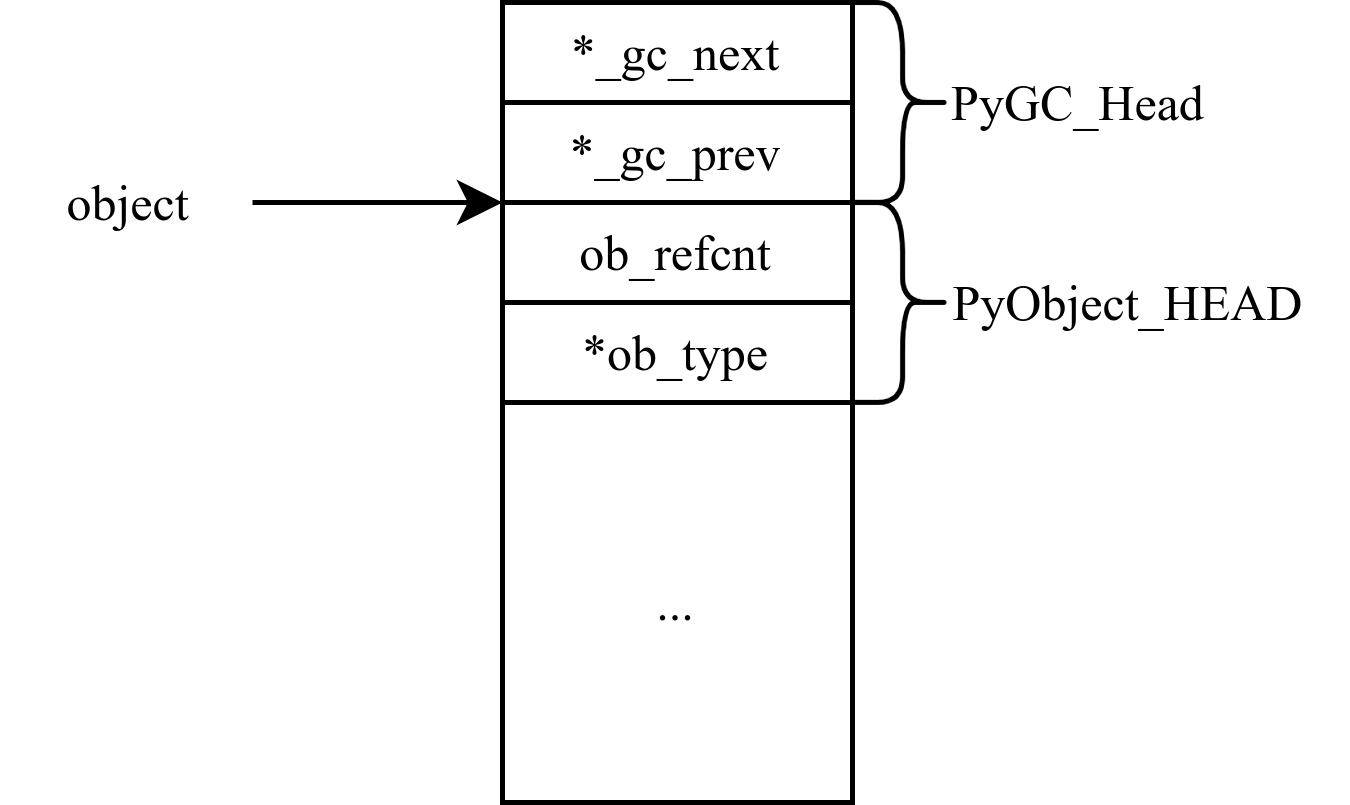
\includegraphics[scale=0.27]{assets/python-object.png}
	\caption{Структура объекта Python}
	\label{fig:pyobject}
\end{figure}

Когда необходима дополнительная информация, связанная со сборщиком мусора, к полям PyGC\_Head можно получить доступ с помощью адресной арифметики и приведения типа исходного объекта.~\cite{python_gc}

Двусвязные списки используются по той причине, что они эффективно поддерживают операции, наиболее часто используемые при выполнении алгоритма сбора мусора, такие как перемещение объекта из одного раздела в другой, добавление нового объекта, полное удаление объекта, а также разбиение и объединение списков.~\cite{python_gc}

\subsubsection{Сборка мусора}

Основная проблема подсчёта ссылок заключается в том, что он не обрабатывает циклические ссылки. Для её решения используется отдельный сборщик мусора, который занимается только очисткой объектов-контейнеров, то есть объектов, которые могут содержать ссылки на другие объекты.~\cite{python_gc}

Алгоритм сборки мусора, который обрабатывает циклические ссылки, состоит в обходе двусвязного списка объектов и использовании метода пробного удаления~\cite{handbook}: объекты, счётчик ссылок на которые не превышает 1, помещаются в список условно недостижимых. Объекты, которые остались в этом списке после завершения обхода графа объектов, могут быть освобождены.~\cite{python_gc}

Стоит отметить, что такая сборка мусора выполняется конкурентно с мутатором в одном выделенном потоке сборщика, не распределяя работу по сборке на несколько потоков приложения.~\cite{python_threaded_gc}


\subsection{Java}

Java~\cite{java_gc_basics} --- компилируемый язык программирования с сильной статической типизацией. Официально был представлен в 1995 году компанией Sun Microsystems. 

% https://www.oracle.com/webfolder/technetwork/tutorials/obe/java/gc01/index.html
Среда выполнения языка Java (Java Runtime Environment, JRE) состоит из \textbf{виртуальной машины Java} (Java Virtual Machine, JVM), основных классов и вспомогательных библиотек платформы Java. Рассматриваемый язык является кроссплатформенным: приложения, разработанные на Java, компилируются в \textbf{байт-код}, который сохраняется в файлах классов и запускается в JVM. Поэтому программы на языке Java можно запустить на всех аппаратных платформах и операционных системах, для которых реализована JVM.~\cite{java_gc_basics}

Существует множество реализаций JVM.~\cite{java_j9}~\cite{java_codename_one}~\cite{java_graalvm}
% https://eclipse.dev/openj9/
% https://www.codenameone.com/
% https://www.graalvm.org/
Среди них наиболее распространённой является HotSpot JVM, представленная в 1999 году компанией Sun Microsystems.~\cite{java_hotspot} % https://openjdk.org/groups/hotspot/



\subsubsection{Управление памятью}
\label{generations}

% https://openjdk.org/groups/hotspot/docs/StorageManagement.html
Частью JVM является \textbf{менеджер хранилища} (storage manager), который отвечает за управление жизненным циклом объектов Java: выделение новых объектов, сбор недоступных объектов и отправку уведомлений о недоступности по запросу.~\cite{java_storage_management} Из соображений масштабируемости, каждый поток JVM имеет собственную область выделения памяти --- \textbf{буфер выделения потока} (Thread-Local Allocation Buffer, TLAB). Каждый поток может выделять ресурсы из своей TLAB без координации с другими потоками, за исключением случаев, когда ему требуется новая TLAB.~\cite{java_storage_management}

% https://openjdk.org/groups/hotspot/docs/StorageManagement.html
Было замечено, что большинство программ на языке Java следует \textbf{гипотезе поколений}~\cite{handbook}, согласно которой в большинстве случаев <<молодые>> объекты (которые создаются позже), с гораздо большей вероятностью перестают использоваться раньше, чем <<старые>> объекты.. Чтобы учесть это свойство программ при распределении памяти, объекты Java разделяются на три поколения: молодое (young), старое (old) и постоянное (permanent). Управление поколениями может осуществляться по различным алгоритмам. Предполагается, что в молодом поколении будет больше объектов, чем в старом, а также будет выше плотность недоступных объектов.~\cite{java_storage_management}

% https://openjdk.org/groups/hotspot/docs/StorageManagement.html
\textbf{Молодое поколение} должно поддерживать быстрое распределение, при этом ожидается, что большинство этих объектов относительно быстро станет недоступным. При сборе мусора в молодом поколении выявляются все достижимые объекты и копируются в старое поколение. Далее объекты, оставшиеся в молодом поколении, освобождаются.~\cite{java_storage_management}

% https://openjdk.org/groups/hotspot/docs/StorageManagement.html
% https://www.oracle.com/technetwork/java/javase/memorymanagement-whitepaper-150215.pdf
Объекты в \textbf{старом поколении} могут анализироваться сборщиком мусора реже, чем объекты в молодом поколении. Также сборщик мусора в зависимости от выбранной стратегии выполнять копирование и уплотнение объектов.~\cite{java_storage_management}~\cite{java_memory}

% https://openjdk.org/groups/hotspot/docs/StorageManagement.html
Помимо объектов, созданных программой на языке Java, существуют объекты, созданные и используемые JVM. Чтобы не путать их с объектами выполняемой программы, такие объекты выделяют в \textbf{постоянное поколение}. Данное название носит исторический характер и на самом деле объекты в нём не существуют на протяжении всего времени выполнения программы.~\cite{java_storage_management} Начиная с Java 8 постоянное поколение было заменено \textbf{метапространством} (MetaSpace), предназначенным для хранения классов и метаданных JVM.~\cite{java_presentation}

\subsubsection{Сборка мусора}

% https://docs.oracle.com/en/java/javase/21/gctuning/available-collectors.html
HotSpot JVM предоставляет несколько сборщиков мусора, оптимизированных для различных типов приложений. Далее будут рассмотрены сборщики мусора, доступные в Java 21.~\cite{java_21_available_collectors}

\textbf{Serial Collector} работает по алгоритму mark-compact (см. п. \ref{tracing}) и использует один поток для выполнения основной и второстепенной работы по сбору мусора, что может повысить его эффективность за счёт отсутствия накладных расходов на взаимодействие параллельных потоков.~\cite{java_21_available_collectors}

\textbf{Parallel Collector} отличается от Serial Collector использованием нескольких потоков для сборки мусора, количество которых может регулироваться с помощью аргументов командной строки.~\cite{java_21_available_collectors} Во время работы Parallel Collector все потоки мутатора приостанавливаются (<<stop the world>>, см. п. \ref{tracing}).~\cite{java_jrockit_memory} Данный сборщик мусора также называют Throughput Collector, так как он может использовать несколько процессоров для ускорения сборки мусора и повышения пропускной способности при работе с памятью, что повышает производительность приложений.~\cite{java_gc_basics}

\textbf{Garbage-First Collector} (также G1) --- это сборщик мусора, работающий по алгоритму mark-sweep (см. п. \ref{tracing}), предназначенный для многопроцессорных машин с большим объемом памяти. Он с высокой вероятностью соответствует целевому времени паузы для сборки мусора, обеспечивая при этом относительно высокую пропускную способность. Операции над всей кучей, такие как глобальная разметка объектов, выполняются конкурентно с потоками приложения. Это предотвращает паузы в работе приложений, пропорциональные размеру кучи и используемых данных. Начиная с версии Java 9, Garbage-First Collector выбирается по умолчанию в большинстве конфигураций оборудования и операционной системы или может быть явно включён с помощью параметров командной строки. Garbage-First Collector достигает высокой производительности при снижении длительности пауз за счет применения следующих методов.~\cite{java_g1}

\begin{enumerate}[label*=\arabic*.]
	\item В отличие от Parallel Collector работа потоков приостанавливается только на некоторые этапы сборки мусора: в начале при разметке объектов из корневого набора (см. п.\ref{tracing}) и в конце при обнаружении изменений, произошедших за время сборки мусора.~\cite{java_jrockit_memory} % https://docs.oracle.com/cd/E15289_01/JRSDK/garbage_collect.htm
	\item Куча разделяется на набор непрерывных областей одинакового размера, называемых регионами. После обнаружения используемых объектов в куче Garbage-First Collector определяет, какие регионы <<почти пусты>> (mostly empty). Именно в этих регионах в первую очередь будет выполняться сбор мусора и уплотнение неиспользуемых объектов, чтобы как можно раньше дать аллокатору непрерывные свободные области памяти наибольшего размера.
	\item Используется \textbf{модель прогнозирования паузы} (pause prediction model) для достижения заданного пользователем целевого времени паузы на сборку мусора и на его основе выбирает количество регионов для обработки.
	\item В отличие от Parallel Collector используемые объекты выбираются для копирования и уплотнения не из всей кучи, а только из некоторых её областей. Эта операция выполняется параллельно на нескольких процессорах, чтобы уменьшить время паузы на сборку мусора и увеличить пропускную способность. Таким образом, при каждой сборке мусора G1 непрерывно работает над уменьшением фрагментации кучи, работая в течение заданного пользователем времени паузы.
\end{enumerate}

\textbf{Z Garbage Collector} (также ZGC) --- это сборщик мусора, работающий по алгоритму mark-compact (см. п. \ref{tracing}) и нацеленный на минимизацию пауз. ZGC работает конкурентно с мутатором, не останавливая выполнение потоков приложения более чем на одну миллисекунду, при этом жертвуя пропускной способностью. Он предназначен для приложений, которым требуется низкая задержка на сборку мусора. Время пауз не зависит от размера используемых данных в куче. ZGC оптимизирован для работы с кучей размером от нескольких сотен мегабайт до 16 Тб.~\cite{java_zgc}

\subsection{Javascript}

JavaScript~\cite{js} --- интерпретируемый язык программирования со слабой динамической типизацией, представленный в 1995 году. Стандартом языка является ECMAScript.~\cite{ecmascript} Наиболее широкое применение JavaScript получил в качестве языка сценариев веб-страниц, но также используется и в других программных продуктах, таких как node.js~\cite{node_js} и Apache CouchDB~\cite{couchdb}.

\textbf{Модель времени выполнения} (runtime model) в JavaScript основана на \textbf{цикле событий} (event loop), который отвечает за сбор и обработку событий, а также за выполнение подзадач из очереди (queued sub-tasks).~\cite{js_event_loop}

Изначально интерпретаторы JavaScript использовали сборку мусора на основе подсчёта ссылок, не обрабатывая циклические ссылки, что могло приводить к систематическим утечкам памяти. По этой причине, начиная с 2012 года, все современные веб-браузеры оснащаются сборщиками мусора, работающими исключительно по алгоритму mark-sweep (см. п. \ref{tracing}). Все усовершенствования алгоритма сборки мусора в интерпретаторах JavaScript (инкрементальная, конкурентная и параллельная сборка мусора, а также применение алгоритма поколений) за последние несколько лет представляют собой усовершенствования данного алгоритма, не являясь новыми алгоритмами сборки мусора, поскольку дальнейшее сужение понятия <<объект более не используется>> не представляется возможным.~\cite{js_memory}

\subsection{C\#}

C\#~\cite{dotnet_tour} --- компилируемый язык программирования с сильной статической типизацией. Официально был представлен в 2001 году компанией Microsoft.

Программы на языке C\# предназначены для запуска на виртуальной среде выполнения \textbf{.NET}, работающей с \textbf{общеязыковой средой выполнения} (Common Language Runtime, CLR) и набором библиотек классов. Среда CLR --- это реализация \textbf{общеязыковой инфраструктуры языка} (Common Language Infrastructure, CLI), являющейся международным стандартом компании Microsoft.~\cite{dotnet_tour} Основные функции среды CLR:~\cite{dotnet_intro}~\cite{dotnet_clr_intro}
% https://github.com/dotnet/runtime/blob/main/docs/design/coreclr/botr/intro-to-clr.md

\begin{itemize}[label*=---]
	\item сборка мусора;
	\item обеспечение безопасности памяти и типов данных;
	\item поддержка языков программирования высокого уровня: C\#, F\# и Visual Basic;
	\item изоляция программ.
\end{itemize}

\subsubsection{Управление памятью}
\label{loh}

% https://learn.microsoft.com/en-us/dotnet/standard/garbage-collection/fundamentals
Сборщик мусора среды Common Language Runtime управляет выделением и освобождением памяти для приложения. При инициализации нового процесса среда выполнения резервирует для него непрерывную область адресного пространства, называемого \textbf{управляемой кучей} (managed heap), которая является частью кучи адресного пространства процесса и предназначена для размещения всех ссылочных типов данных. Выделение памяти из управляемой кучи происходит быстрее, чем неуправляемое выделение памяти, так как среда выполнения выделяет память путём изменения указателя на следующий объект в куче, что аналогично выделению памяти на стеке. Кроме того, последовательно хранение объектов позволяет ускорить доступ к ним. Также стоит отметить, что все потоки процесса выделяют память в одной куче.~\cite{dotnet_memory}

% https://learn.microsoft.com/en-us/dotnet/standard/garbage-collection/large-object-heap
Для повышения производительности среда выполнения выделяет память для больших объектов (размером не менее 85 000 байт) в отдельной куче, называемой \textbf{кучей больших объектов} (Large Object heap, LOH). Также во избежание перемещения больших объектов в памяти куча больших объектов, как правило, не подлежит уплотнению.~\cite{dotnet_loh}



\subsubsection{Сборка мусора}

% https://learn.microsoft.com/en-us/dotnet/standard/garbage-collection/fundamentals
Сборщик мусора определяет оптимальное время для выполнения сбора на основе выделяемых ресурсов. Перед началом сборки мусора все управляемые потоки приостанавливаются, за исключением потока, который инициировал сборку. Период времени, в течение которого сборщик мусора активен, называется его \textbf{задержкой} (delay). Сборщик мусора работает по алгоритму mark-compact (см. п. \ref{tracing}), разделяя сбор мусора на три фазы.~\cite{dotnet_gc}

\begin{enumerate}[label*=\arabic*.]
	\item \textbf{Фаза разметки}: определение неиспользуемых объектов путём исследования корневого набора программы (см. п. \ref{roots}), каждый элемент которого либо ссылается на объект в управляемой куче, либо имеет значение null. Корневой набор включает статические поля, локальные переменные и параметры в стеке потока, а также регистры процессора. Сборщик мусора имеет доступ к списку активных <<корней>>, который поддерживается JIT-компилятором и средой выполнения. С помощью этого списка исследуется корневой набор и строится граф доступных объектов.
	\item \textbf{Фаза перемещения}: корректировка указателей, чтобы после сжатия используемых данных элементы корневого набора ссылались на новое местоположение объектов.
	\item \textbf{Фаза уплотнения}: освобождение объектов, которые не попали в граф на этапе разметки, считаются недоступными и освобождаются. На данном этапе сборщик мусора проверяет управляемую кучу в поисках областей памяти, занятых недоступными объектами. При обнаружении каждого недостижимого объекта он использует функцию копирования для уплотнения доступных объектов, тем самым освобождая области памяти, выделенные для недоступных объектов. Он также устанавливает указатель управляемой кучи за последним доступным объектом. 
\end{enumerate}

% https://learn.microsoft.com/en-us/dotnet/standard/garbage-collection/fundamentals
Сбор мусора гарантированно происходит при выполнении одного из следующих условий.~\cite{dotnet_gc}

\begin{enumerate}[label*=\arabic*.]
	\item В системе обнаружена нехватка физической памяти. Данная ситуация определяется либо по уведомлению от операционной системы, либо по приближении к пределу объёма физической памяти, доступной на вычислительной машине.
	\item Объём памяти, используемый объектами в управляемой куче, превысил допустимое пороговое значение, которое может корректироваться во время выполнения программы.
	\item Сборщик мусора вызван явно с помощью метода GC.Collect.
\end{enumerate}

% https://learn.microsoft.com/en-us/dotnet/standard/garbage-collection/fundamentals
Работа сборщика мусора основана на следующих соображениях.~\cite{dotnet_gc}

\begin{itemize}[label*=---]
	\item Уплотнение для части управляемой кучи выполняется быстрее, чем для всей управляемой кучи.
	\item Новые объекты, как правило, обладают меньшим временем жизни по сравнению со старыми объектами.
	\item Новые объекты, как правило, связаны друг с другом и используются приложением примерно в одно и то же время.
\end{itemize}

Для повышения производительности сборщика мусора и снижения среднего времени паузы на сборку, управляемая куча разделена на три поколения, обрабатываемые отдельно. Поскольку сжать часть управляемой кучи быстрее, чем всю кучу, эта схема позволяет сборщику мусора освобождать память только в определенном поколении, а не во всей управляемой куче при каждом вызове.~\cite{dotnet_gc}~\cite{dotnet_memory}

\textbf{Поколение 0} содержит самые новые и, как правило, недолговечные объекты, такие как локальные переменные. Сбор мусора происходит чаще всего именно в этом поколении, при этом зачастую освобождается достаточно памяти, чтобы приложение могло продолжать выделять память. Объекты, оставшиеся после сборки мусора поколения 0, переводятся в поколение 1.

\textbf{Поколение 1} служит буфером между новыми и старыми объектами. Если сбор мусора в поколении 0 не освобождает достаточно памяти для того, чтобы приложение могло создать новый объект, сборщик мусора может выполнить сборку в поколении 1, а затем в поколении 2. Объекты, оставшиеся после сборки мусора поколения 1, переводятся в поколение 2.

\textbf{Поколение 2} содержит старые объекты, такие как статические данные, используемые на протяжении всего времени выполнения программы. Объекты, попавшие в поколение 2, остаются в нём до тех пор, пока они не перестанут использоваться в программе. Также при сборе мусора в поколении 2 выполняется сбор объектов в куче больших объектов (иногда называется поколением 3).

\subsection{Golang}

Golang (также Go)~\cite{golang} --- компилируемый язык программирования с сильной статической типизацией, разработанный компанией Google. Официально язык был представлен в ноябре 2009 года.

В любой программе на языке Golang присутствует \textbf{среда выполнения} (runtime)~\cite{golang_runtime}, то есть код, который выполняется без ведома программиста. Среда выполнения состоит из следующих компонентов.

\begin{enumerate}[label*=\arabic*.]
	\item \textbf{Планировщик} (Sheduler)~\cite{golang_scheduler}, отвечающий за управление работой горутин. \textbf{Горутина} --- это легковесный поток, управляемый средой выполнения языка Golang.~\cite{golang_goroutine}
	\item \textbf{Аллокатор памяти}.
	\item \textbf{Сборщик мусора}.
\end{enumerate}

\subsubsection{Структура кучи}

Куча состоит из набора областей, называемых \textbf{аренами} (Arena), размер которых составляет 64 Мб в 64-разрядной версии и 4 Мб в 32-разрядной (heapArenaBytes). Начальный адрес каждой арены также выровнен по размеру арены.  С каждой ареной связан объект heapArena~\cite{golang_mheap}, который хранит метаданные для этой арены: битовую карту кучи для всех слов (word) в арене и карту span для всех страниц в ней. Объекты heapArena выделяются вне кучи. Структура mheap содержит \textbf{карту арен}, которая охватывает всё доступное адресное пространство программы, поэтому его можно рассматривать как набор арен. Аллокатор старается сохранять арены смежными, чтобы большие span (и, следовательно, большие объекты) могли занимать одновременно несколько арен.~\cite{golang_malloc}

\subsubsection{Сборка мусора}

В языке Golang для сборки мусора используется алгоритм \textbf{Concurrent Mark-Sweep}, являющийся модификацией алгоритма mark-sweep (см. п. \ref{tracing}), предназначенного для конкурентной сборки мусора. Сборщик мусора запускается параллельно с мутатором и позволяет нескольким потокам сборки мусора выполняться параллельно. Алгоритм сборки мусора не является уплотняющим и не использует поколения (см. п. \ref{generations}).~\cite{golang_gc}

Сборщик мусора языка Golang использует трёхцветную абстракцию, в рамках которой граф объектов разбивается на черные (предположительно используемые) и белые (возможно, неиспользуемые) объекты. Изначально каждый объект белый. Когда объект впервые обнаруживается во время трассировки, он окрашивается в серый цвет. Когда объект был отсканирован и были идентифицированы его дочерние элементы, он закрашивается чёрным.~\cite{handbook}

Для конкурентной разметки и очистки используются \textbf{барьеры записи} (write barrier), позволяющий избежать ситуации, когда чёрные объекты указывают на белые. Такое может произойти, например, при перемещении указателя в программе до того, как сборщик мусора успел его разметить. В такой ситуации мутатор скрывает объект от сборщика мусора.~\cite{golang_gc} Для реализации барьера записи используются операции <<затенения>> (shade), перемещающие указатели программы. Барьер записи <<затеняет>> как записываемый указатель, так и записываемое значение при любой записи по указателю~\cite{golang_barrier}. 

Ниже представлено описание основных шагов алгоритма сборки мусора.~\cite{golang_gc}

\begin{enumerate}[label*=\arabic*.]
	\item Фаза завершения очистки (sweep termination).
	\begin{enumerate}[label*=\arabic*.]
		\item <<Остановка мира>> (<<stop the world>>, см. п. \ref{tracing}), приводящая к тому, что все потоки достигают \textbf{безопасной точки} (GC safe-point).
		\item Очистка всех мусорных mspan. Неочищенные mspan будут только в том случае, если цикл сборки мусора был запущен раньше ожидаемого времени.
	\end{enumerate}
	
	\item Фаза разметки (mark).
	\begin{enumerate}[label*=\arabic*.]
		\item Включение барьера записи, постановка в очередь заданий по разметке объектов из корневого набора (см. п. \ref{tracing}) и включение ассистентов (assistants), выполняющих свою работу во время выделения памяти. Никакие объекты не могут быть просканированы до тех пор, пока все потоки не включат барьер записи, что достигается с помощью <<остановки мира>>.
		\item <<Запуск мира>> (<<start the world>>). С этого момента работа сборщика мусора выполняется обработчиками разметки (mark workers), запущенными планировщиком, и ассистентами. Выделяемые объекты отмечаются чёрным цветом.
		\item Разметка объектов из корневого набора, включающая в себя сканирование стеков всех горутин, <<затенение>> всех глобальных переменных и любых указателей кучи в структурах данных среды выполнения вне кучи. При сканировании стека горутина останавливается, <<затеняются>> все указатели, найденные в её стеке, а затем горутина продолжает выполняться.
		\item Очистка рабочей очереди от серых объектов. Каждый серый объект сканируется и отмечается чёрным, <<затеняя>> все указатели, найденные в объекте, что, в свою очередь, может привести к добавлению этих указателей в рабочую очередь.
		\item Выполнение алгоритма распределенного завершения (distributed termination algorithm), чтобы определить, когда закончится выполнение заданий разметки объектов из корневого набора или серых объектов.
	\end{enumerate}
	
	\item Фаза завершения разметки (mark termination).
	\begin{enumerate}[label*=\arabic*.]
		\item <<Остановка мира>>.
		\item Отключение обработчиков и ассистентов.
		\item Очистка, включающая сброс кешей mcache.
	\end{enumerate}
	
	\item Фаза очистки (sweep).
	\begin{enumerate}[label*=\arabic*.]
		\item Отключение барьера записи.
		\item <<Запуск мира>>. С этого момента выделяемые объекты становятся белыми. Также при необходимости аллокатор может очищать mspan перед использованием.
		\item Выполнение параллельной очистки в фоновом режиме и во время выделения памяти.
	\end{enumerate}
\end{enumerate}

\subsection{Классификация существующих решений}

Ниже приведены критерии классификации алгоритмов распределения памяти.

\begin{enumerate}[label*=\arabic*.]
	\item \textbf{Разделение объектов на поколения}. \newline
	Для оптимизации сборки мусора и уменьшения времени пауз в языках программирования может использоваться алгоритм поколений (см. п. \ref{generations}). В таблице сравнения будут использоваться обозначения <<+>> и <<->> для определения использования алгоритма поколений менеджером памяти рассматриваемого языка программирования.
	
	\item \textbf{Отсутствие хранения вспомогательных данных в объектах}. \newline
	Для реализации алгоритмов распределения памяти может понадобиться хранение дополнительных данных в выделяемых объектах, что создаёт зависимость объёма памяти, необходимого сборщику мусора, от количества отслеживаемых объектов. В таблице сравнения для обозначения факта хранения вспомогательных данных в объектах будет использоваться <<->>, иначе --- <<+>>.
	
	\item \textbf{Использование конкурентной сборки мусора}. \newline
	Для снижения времени пауз на сборку мусора менеджеры памяти некоторых языков программирования могут выполнять её конкурентно с потоками мутатора. В таблице сравнения для обозначения факта использования конкурентной сборки мусора будет использоваться <<+>>, иначе --- <<->>.
	
	\item \textbf{Использование параллельной сборки мусора}. \newline
	Менеджеры памяти некоторых языков программирования могут выполнять сборку мусора параллельно в нескольких потоках приложения, задействуя больше вычислительных ресурсов процессора для её ускорения. В таблице сравнения для обозначения факта использования параллельной сборки мусора будет использоваться <<+>>, иначе --- <<->>.
	
	\item \textbf{Отсутствие остановки потоков мутатора на весь цикл сборки мусора}. \newline
	Некоторые алгоритмы сборки мусора оптимизированы таким образом, чтобы останавливать работу потоков основной программы только на некоторых этапах сбора для минимизации времени пауз. В таблице сравнения для обозначения этого факта будет использоваться <<+>>, иначе --- <<->>.
	
	\item \textbf{Количество остановок потоков мутатора за один цикл сборки мусора}.
\end{enumerate}

Описанные выше характеристики алгоритмов распределения памяти, как правило, декларируются в документациях к соответствующим языкам программирования. Результаты сравнения алгоритмов распределения памяти приведены в таблице \ref{tab:compare}.

\begin{table}[H]
	\centering
	\caption{Сравнение алгоритмов распределения памяти}
	\label{tab:compare}
	\begin{tabular}{|c|c|c|c|c|c|c|c|}
		\hline
		\rotatebox[origin=l]{90}{\parbox[l]{8cm}{Язык программирования}} 
		& \rotatebox[origin=l]{90}{\parbox[l]{8cm}{Сборщик мусора}} 
		& \rotatebox[origin=l]{90}{\parbox[l]{8.8cm}{Разделение объектов на поколения}} 
		& \rotatebox[origin=l]{90}{\parbox[l]{8.8cm}{Отсутствие хранения вспомогательных данных в объектах}} 
		& \rotatebox[origin=l]{90}{\parbox[l]{8.2cm}{Использование конкурентной сборки мусора}} 
		& \rotatebox[origin=l]{90}{\parbox[l]{8.2cm}{Использование параллельной сборки мусора}} 
		& \rotatebox[origin=l]{90}{\parbox[l]{9.1cm}{Отсутствие остановки потоков мутатора на весь цикл сборки мусора}} 
		& \rotatebox[origin=l]{90}{\parbox[l]{9.1cm}{Количество остановок потоков мутатора за один цикл сборки мусора}} 
		\\ \hline
		Python & По умолчанию 			& + & - & + & - & + & 1 \\ \hline
		\multirow{4}{*}{Java} & Serial 	& + & + & + & - & - & 1 \\ \cline{2-8}
		& Parallel 					& + & + & + & + & - & 1 \\ \cline{2-8}
		& Garbage-First 				& + & + & + & + & + & 2 \\ \cline{2-8}
		& ZGC 							& + & + & + & + & + & 1 \\ \hline
		JavaScript & По умолчанию 		& - & + & - & - & - & 1 \\ \hline
		C\# & По умолчанию 				& + & + & + & + & - & 1 \\ \hline
		Golang & По умолчанию 			& - & + & + & + & + & 2 \\ \hline
	\end{tabular}
\end{table}

Среди рассмотренных интерпретируемых языков программирования наиболее оптимизированным для различных сценариев использования можно считать менеджер памяти языка Python за счёт применения алгоритма поколений и подсчёта ссылок.

Среди рассмотренных компилируемых языков программирования наиболее универсальным и масштабируемым можно считать менеджер памяти языка Java за счёт предоставления пользователю возможности выбора сборщика мусора для выполнения каждой программы, а также оптимизации времени пауз на сборку мусора.



\section{Классификация алгоритмов по требованиям к дополнительной памяти}

Теоретическое исследование ресурсных характеристик компьютерных алгоритмов предполагает введение соответствующих классификаций, отражающих различные ресурсные требования алгоритма и его программной реализации.~\cite{uljanov}

Далее будет рассмотрена классификация компьютерных алгоритмов, в основу которой положен требуемый алгоритмом объём дополнительной памяти в принятой модели вычислений. В данном случае рассматривается только объём оперативной
памяти, так как затраты памяти на внешних носителях требуют отдельного рассмотрения и выходят за рамки работы. Пусть $D$ --- конкретный вход алгоритма $A$, причем $|D| = n$, где $n$ --- длина или некоторая мера длины входа. Под объёмом памяти, требуемым алгоритмом $A$ для входа, заданного множеством $D$, будем понимать максимальный объём памяти модели вычислений, задействованный в ходе выполнения алгоритма. Функцию объёма памяти алгоритма для входа $D$ будем обозначать через $V_A(D)$. Значение функции $V_A(D)$ есть целое положительное число.~\cite{uljanov}

Ресурсные требования алгоритма к объёму памяти определяются памятью входа, выхода и дополнительной памятью, задействованной алгоритмом в ходе его выполнения. В соответствии с этим будем различать следующие компоненты функции объема памяти: память входа $V_I(D)$, память выхода $V_R(D)$ и дополнительная память $V_t(D)$. По объёму памяти входа (выхода) алгоритмы можно разделить на потоковые, обрабатывающие входные (выходные) данные поэлементно, и непотоковые, хранящие входные (выходные) данные в памяти целиком.~\cite{uljanov}

Поскольку ресурсные компоненты $V_I(D)$ и $V_R(D)$ во многом определяются особенностями задачи, а для различных алгоритмов ее решения, обладающих статическими входом и выходом, фактически совпадают, то именно компонент $V_t(D)$ различает алгоритмы по ресурсным затратам памяти в рамках статического или потокового типа. Очевидно, что для современных компьютеров ограничение решаемых задач по ресурсу оперативной памяти не столь существенно, как ограничения по временной эффективности. Тем не менее известная дилемма «память-время» приводит к тому, что попытка улучшения временных характеристик приводит к ощутимым затратам памяти, даже при современных объемах. Актуальные размерности современных сложных задач также приводят к тому, что ресурс памяти становится значимым в комплексной оценке ресурсной эффективности алгоритма. Однако при сравнении алгоритмов, относящихся или к статическому, или к потоковому типу, основную роль играет именно дополнительная память, затраты которой обусловлены спецификой данного алгоритма. В связи с этим предлагается следующая классификация алгоритмов, основанная на оценке дополнительной памяти.~\cite{uljanov}

\textbf{Класс V0} --- алгоритмы с нулевой дополнительной памятью.
\begin{equation}
	\forall n > 0, \forall D \in D_n ~~V_t(D) = 0.
\end{equation}
Алгоритмы этого класса либо вообще не требуют дополнительной памяти, либо используют ресурсы памяти входа и/или выхода в качестве необходимой дополнительной памяти по мере обработки элементов входа или по мере заполнения памяти результата.~\cite{uljanov}

\textbf{Класс VC} --- алгоритмы с фиксированной дополнительной памятью.
\begin{equation}
	\forall n > 0, \forall D \in D_n ~~	V_t(D) = const \neq 0.
\end{equation}
Алгоритмы класса $VC$ используют постоянный, не зависящий от длины и особенностей входа и длины выхода, объём дополнительной оперативной памяти. В реальных алгоритмах --- это, как правило, память для хранения счетчиков циклов, промежуточных результатов вычислений и указателей на структуры.~\cite{uljanov}

\textbf{Класс VL} --- алгоритмы, дополнительная память которых линейно зависит от длины входа. Введём в рассмотрение функцию дополнительной памяти в худшем случае для всех допустимых входов с мерой $n$, обозначив её через $V\hat{_t}(n)$:
\begin{equation}
	V\hat{_t}(n) = \max_{D \in D_n}V_t(D).
\end{equation}
В этих обозначениях алгоритм принадлежит к типу с линейной дополнительной памятью, если
\begin{equation}
	V\hat{_t}(n) = \Theta(n),
\end{equation}
где обозначение Θ есть стандартное обозначение класса функций в асимптотическом анализе.~\cite{uljanov}

\textbf{Класс VQ} --- алгоритмы, дополнительная память которых квадратично зависит от длины входа. Для этого типа алгоритмов объём дополнительной памяти в худшем случае для входов размерности $n$ пропорционален по порядку квадрату меры размерности:
\begin{equation}
	V\hat{_t}(n) = \Theta(n^2).
\end{equation}
Примером может служить стандартный алгоритм умножения длинных целых чисел, заданных побитно массивами длины $n$.~\cite{uljanov}

\textbf{Класс VP} --- алгоритмы, дополнительная память которых имеет полиномиальную надквадратичную зависимость. Это алгоритмы, требующие ресурса дополнительной памяти, по порядку большего, чем квадрат меры длины входа, но полиномиально зависящего от этой меры:
\begin{equation}
	\exists k > 2: V\hat{_t}(n) = \Theta(n^k).
\end{equation}	
К этому классу относятся, например, рекурсивные алгоритмы, порождающие дерево рекурсии с оценкой глубины $\Theta(n^k), k > 1$, и требующие хранения в каждой вершине дерева дополнительного массива, имеющего длину порядка $\Theta(n)$.~\cite{uljanov}

\textbf{Класс VE} --- алгоритмы, дополнительная память которых экспоненциально зависит от длины входа. Формально это тип алгоритмов, требующих, в худшем случае, ресурса дополнительной памяти, по порядку экспоненциально зависящего от меры длины входа:
\begin{equation}
	\exists \lambda > 0: V\hat{_t}(n) = \Theta(e^{\lambda n}).
\end{equation}
Реально это алгоритмы, использующие дополнительные массивы или более сложные структуры данных, размер которых определяется значениями элементов входа. Характерным примером могут служить алгоритм сортировки методом индексов или табличные алгоритмы, реализующие метод динамического программирования.~\cite{uljanov}


\section{Постановка задачи}

Алгоритмы автоматического управления памятью в каждом из языков программирования обладают различными недостатками, среди которых однопоточная или неконкурентная сборка мусора, необходимость остановки потоков мутатора для её выполнения, а также отсутствие разделения объектов на поколения. Поэтому разрабатываемый метод должен быть ориентирован на устранение недостатков существующих решений, возникающих при реализации алгоритмов, относящихся к классам VL, VQ, VP, VE, а также VC при условии, что дополнительная память для работы такого алгоритма будет выделяться в куче, а не на стеке (например, во избежание переполнения стека).

На рисунке \ref{fig:idef0} представлена диаграмма IDEF0 нулевого уровня решаемой задачи.

\begin{figure}[H]
	\centering
	\includegraphics[width=\textwidth]{assets/idef0.png}
	\caption{Диаграмма IDEF0 нулевого уровня}
	\label{fig:idef0}
\end{figure}

Под временем выполнения метода понимается время, которое пользовательская программа затрачивает на вызовы реализации метода, то есть на выделение памяти и обращение к выделенным объектам. Гарантия времени выполнения метода подразумевает, что это время будет иметь некоторое ограничение, выражаемое асимптотической оценкой сложности алгоритмов выделения памяти и обращения к ней.

Подсчёт ссылок позволяет при освобождении памяти распределять накладные расходы по всему времени работы программы. При этом сбор циклических ссылок должен осуществляться конкурентно с основной программой, чтобы снизить накладные расходы мутатора на работу с объектами.



\section*{Выводы из аналитического раздела}

В данном разделе был проведён анализ предметной области автоматического управления памятью. Были проведены анализ и классификация существующих решений. На основе классификации методов была сформулирована концепция комбинированного метода и обозначена область его применения. Постановка задачи была формализована в виде функциональной схемы метода в нотации IDEF0.
